\chapter{Projektowanie aplikacji}
Proces projektowania aplikacji jest fazą, w której planowane są kwestie jak ma zostać zbudowana aplikacja, aby spełnić wszystkie wcześniej założone wymagania funkcjonalne oraz niefunkcjonalne. 

\section{Model informacyjny}
Na podstawie założeń zawartych w poprzednich rozdziałach został zaprojektowany model informacyjny zaprezentowany na Rysunku \ref{fig:db}. Będzie on niezbędny w implementacji bazy danych.

\begin{figure}[H]
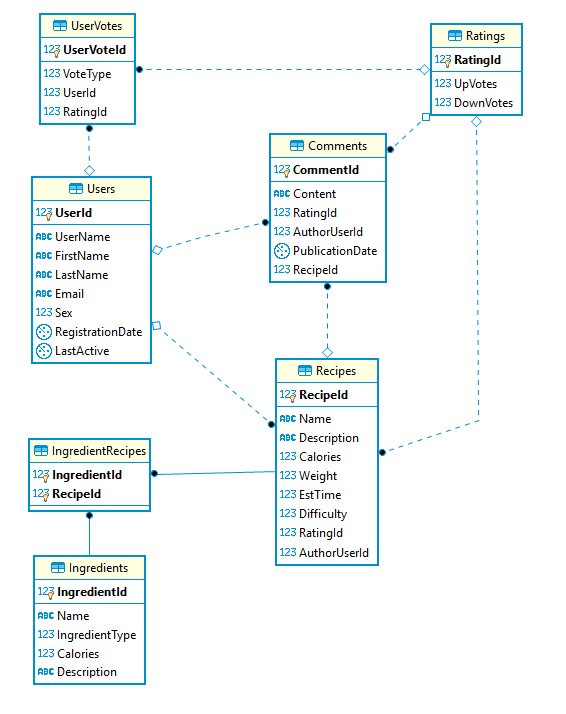
\includegraphics[width=\textwidth]{rys/db.png}
\caption{Model informacyjny aplikacji}
\label{fig:db}
\end{figure}

Najważniejszym elementem schematu jest przepis (encja \textit{Recipes}), który zawiera nazwę i opis w postaci tekstowej. Poza tym zawiera liczbę kalorii, wagę, szacowany czas w postaci liczb. Poziom trudności jest typem wyliczeniowym, więc w bazie danych będzie de facto przechowywany w postaci liczby. Kolejnym bardzo ważnym elementem są klucze obce do encji użytkownika oraz oceny.\newline
Następnym elementem jest ocena (encja \textit{Ratings}), która zawiera głosy negatywne oraz pozytywne.\newline
Kolejny jest komentarz (encja \textit{Comments}), która zawiera treść w postaci tekstu, datę publikacji, klucz obcy do autora wpisu, oceny oraz przepisu, do którego się odwołuje.\newline
Następnym elementem jest głos użytkownika (encja \textit{UserVotes}), który zawiera w sobie rodzaj głosu (negatywny lub pozytywny) i klucze obce do użytkownika, który oddał głos oraz do oceny, do której się odnosi.\newline
Dalszym w kolejności elementem jest użytkownik (encja \textit{Users}), który przechowuje szczegóły dotyczące użytkownika, takie jak nazwa użytkownika, imię, nazwisko, email, płeć, datę rejestracji oraz ostatnią aktywność. Nie przechowuje za to haseł, ponieważ powinny być przechowywane oddzielnie od danych aplikacji.\newline
Kolejnym elementem jest składnik (encja \textit{Ingredients}. Zawiera on w sobie nazwę, typ składnika, liczbę kalorii na 100 gramów oraz opis.\newline
Między przepisami, a składnikami występuje relacja wiele do wielu, aby możliwa była późniejsza implementacja tej struktury, potrzebna jest dodatkowa encja wiążąca je razem. Nazwana została \textit{IngredientRecipes} i łączy ona klucze składników z kluczami przepisów.

\section{Architektura logiczna}
\label{chap:arch_log}
Architektura logiczna aplikacji w głównej mierze wynika z technologii, która została użyta w implementacji. Na Rysunku \ref{fig:arch_log} została przedstawiony jej schemat. Warstwa logiki została wyraźnie oddzielona od warstwy klienta.\newline

\begin{figure}[H]
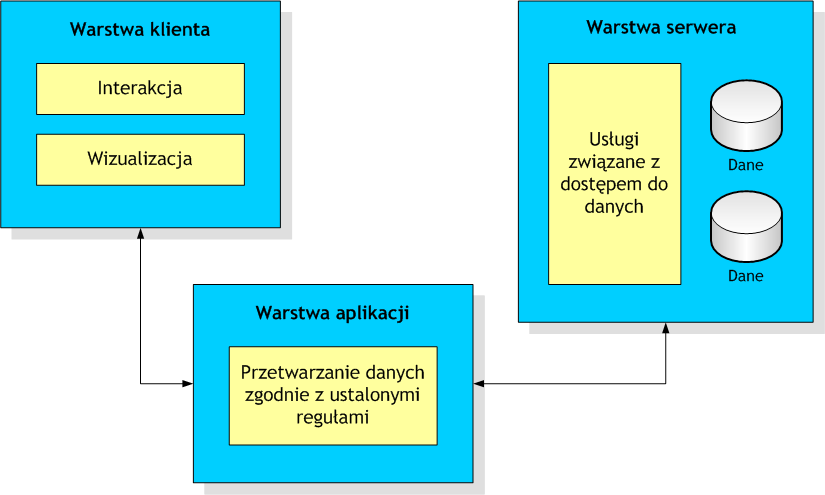
\includegraphics[width=\textwidth]{rys/arch-logiczna.png}
\caption{Architektura logiczna aplikacji}
\label{fig:arch_log}
\end{figure}

Warstwa klienta ma za zadanie wizualizować i prezentować użytkownikowi dane. Poza tym musi pozwalać na interakcję. W takiej postaci klient pełni rolę tzw. forntendu.\newline
Warstwa aplikacji pełni swoisty pomost między bazą danych, a klientem. Ma za zadanie pobierać i przetwarzać dane (np. filtrować, walidować), a także dostarczać nowe porcje danych do bazy danych. Tutaj też powinna znajdować się cała logika biznesowa jak i funkcjonalność odpowiedzialna za liczenie. \newline
Warstwą serwera jest dowolnie wybrana implementacja bazy danych. Ma za zadanie przechowywać dane aplikacji oraz dane kont użytkowników. W tym miejscu można było się pokusić o wybranie nierelacyjnej bazy danych, lecz ostatecznie została wybrana relacyjna.

\section{Architektura fizyczna}
\label{chap:arch_fiz}
Na Rysunku \ref{fig:arch_fiz} został przedstawiony schemat architektury fizycznej aplikacji. Bliźniaczo jak w przypadku architektury logicznej jej struktura narzucona jest wyborami technologii przedstawionych w Rozdziale \ref{chap:technologies}. Składają się one z backendu .NET Core, który używa GraphQL jako standardu API. Zarządza on bazami danych postawionych na PostgreSQL. Rolę klienta pełni środowisko programistyczne Angular posiadające komponenty, które zawierają logikę aplikacji frontendowej i komunikują się z widokami. Poprzez wstrzykiwanie zależności komponenty mają dostęp do wspólnych zasobów i funkcji. Aplikacja klienta posiada również możliwości zapisywania danych w przeglądarce użytkownika w postaci ciasteczek, co może być przydatne przy zapisywaniu aktualnego stanu zalogowanego użytkownika.


\begin{figure}[H]
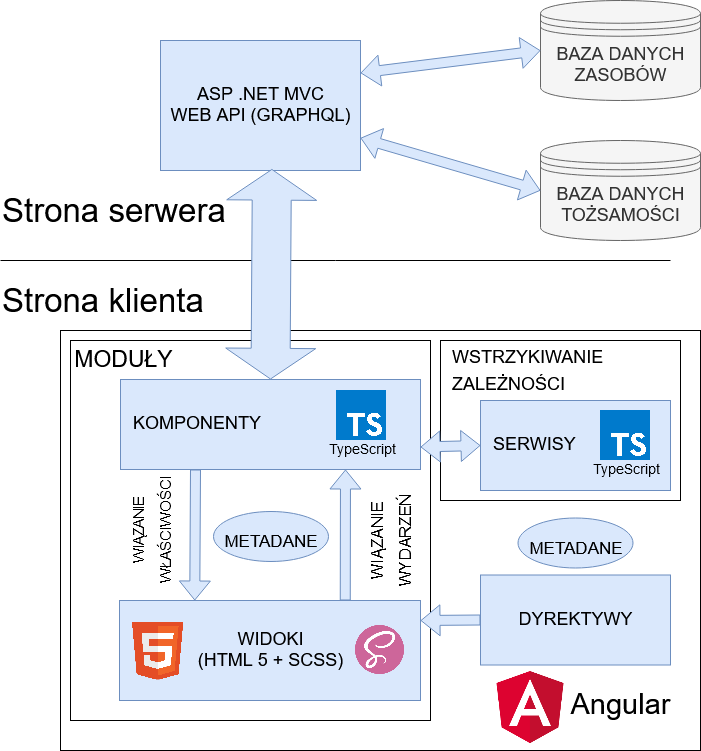
\includegraphics[width=\textwidth]{rys/arch-fiz.png}
\caption{Architektura fizyczna aplikacji}
\label{fig:arch_fiz}
\end{figure}


